Los datos utilizados provienen de la competición Crowdsensing-based Road Damage Detection Challenge (CRDDC2022). Se trata de un conjunto de datos con imágenes de carreteras y aceras, etiquetadas con la presencia de daños en el pavimento. Los datos provienen de seis países: China, República Checa, India, Japón, Noruega y Estados Unidos. Cada uno de estos países tiene un conjunto de datos que consiste en imágenes de carreteras tomadas desde un vehículo en movimiento. Además, China también proporciona un conjunto de datos con imágenes tomadas desde un dron, sumando un total de siete conjuntos de datos. Estos conjuntos de datos se dividen a su vez en entrenamiento y test, donde el conjunto de entrenamiento se compone de imágenes con sus respectivas etiquetas de daños en el pavimento, y el conjunto de test se compone de imágenes sin etiquetar. Las etiquetas de daños en el pavimento se proporcionan en forma de coordenadas de caja delimitadora (bounding box) y una etiqueta que representa el tipo de daño asociado a la caja. 

Los organizadores de la competición han publicado un paper \cite{RDD2022_data_paper} donde se detallan los datos y se proporciona una descripción de los mismos. En esta sección se va a hacer un resumen de los datos y se va a explicar cómo se estructuran, qué información contienen y cómo son las imágenes.


\subsection{¿Cómo descargar los datos?}
En el repositorio de la competición \cite{RoadDamageDetector_repo} se proporciona un README con una sección sobre los datos de la CRDDC2022. En esta sección del README se pueden descargar zips con los datos completos y por país. Además, se proporciona un enlace a figshare \cite{RDD2022_dataset} donde se pueden descargar los datos completos. Personalmente, tuve problemas descargando los datos desde estas fuentes, ya que los datos correspondientes a Noruega me llegaban corruptos. Es por esto que opte por descargar los datos desde DatasetNinja \cite{RDD2022_datasetNinja}, donde se puede descargar los datos completos sin problemas.


\subsection{¿Cómo se estructuran los datos?}
Los datos de la CRDDC2022 se estructuran en siete carpetas, una por cada uno de los subconjuntos antes mencionados. Cada carpeta contiene dos carpetas, una de train y otra de test. Las carpetas de train tienen otras dos subcarpetas una para las imágenes y otra para los archivos de anotaciones, mientras que las carpetas de test solo tienen una carpeta de imagenes. Las imágenes y sus correspondientes anotaciones se nombran de la misma forma, de manera que se pueda asociar una imagen con su anotación. El formato de estos nombres es \texttt{<región>\_<identificador>.<extension>}, donde \texttt{<región>} es el subconjunto al que pertenece la imagen, \texttt{<identificador>} es un número que identifica a la imagen, y \texttt{<extension>} es la extensión del archivo. Las imágenes son todas en formato \texttt{jpg}, y las anotaciones son en formato \texttt{xml} si se descarga el conjunto por el repositorio de la competición o figshare, y en formato \texttt{json} si se descarga el conjunto por DatasetNinja. En la descarga por DatasetNinja, los datos no estan dividos por subconjunto sino que se encuantran todos juntas en las carpetas generales de train y test.


\subsection{¿Qué información contienen las anotaciones?}
Las anotaciones como hemos dicho pueden venir en formato \texttt{xml} o \texttt{json} dependiendo de la fuente de descarga. No obstante, la información que contienen es la misma. Cada anotación contiene la información de su imagen correspondiente, y esta información se estructura de la siguiente forma:
\begin{itemize}
    \item \texttt{filename}: Nombre de la imagen.
    \item \texttt{size}: Tamaño de la imagen en píxeles.
    \item \texttt{objects}: Lista de objetos en la imagen. Cada objeto contiene:
    \begin{itemize}
        \item \texttt{name}: Nombre de la clase del objeto.
        \item \texttt{bndbox}: Coordenadas de la caja delimitadora del objeto.
    \end{itemize}
\end{itemize}
Es importante mencionar que las coordenadas de la caja delimitadora se proporcionan en formato \texttt{xmin, ymin, xmax, ymax}, donde \texttt{xmin} y \texttt{ymin} son las coordenadas del punto superior izquierdo de la caja, y \texttt{xmax} y \texttt{ymax} son las coordenadas del punto inferior derecho de la caja. Además, las coordenadas se proporcionan en píxeles. Después tendremos que normalizar estas coordenadas y adaptarlas al formato requerido por nuestros modelos para poder trabajar con ellas.

Los datos originales contienen hasta 11 clases distintas de etiquetas de daños en el pavimento. Estas clases son: \texttt{D00, D20, D10, D40, D44, D50, D43, D01, D11, Repair, Block Crack}. No obstante, en la competición solo se consideran las cuatro primeras clases, que son las más comunes y resumen la mayoría de los daños en el pavimento. Estas clases tienen los siguientes significados:

\begin{itemize}
    \item \texttt{D00}: Longitudinal crack o grieta longitudinal.
    \item \texttt{D10}: Transverse crack o grieta transversal.
    \item \texttt{D20}: Alligator crack o grieta de cocodrilo.
    \item \texttt{D40}: Pothole o bache.
\end{itemize}

El conjunto de datos de descargado de DatasetNinja tiene la ventaja de que ya agrupa todas las clases que se van a ignorar en la competición en una sola clase llamada \texttt{Other Corruption}. Esto facilita el trabajo con los datos, ya que no es necesario hacer esta agrupación manualmente. En la figura \ref{fig:datasetNinja_class_count_bar} se puede ver el número de anotaciones por clase en los datos de la CRDDC2022.

% Añadimos las gráficas daatasetNinja_class_count_bar y datasetNinja_class_distribution_pie de la carpeta graphs
\begin{figure}[H]
    \centering
    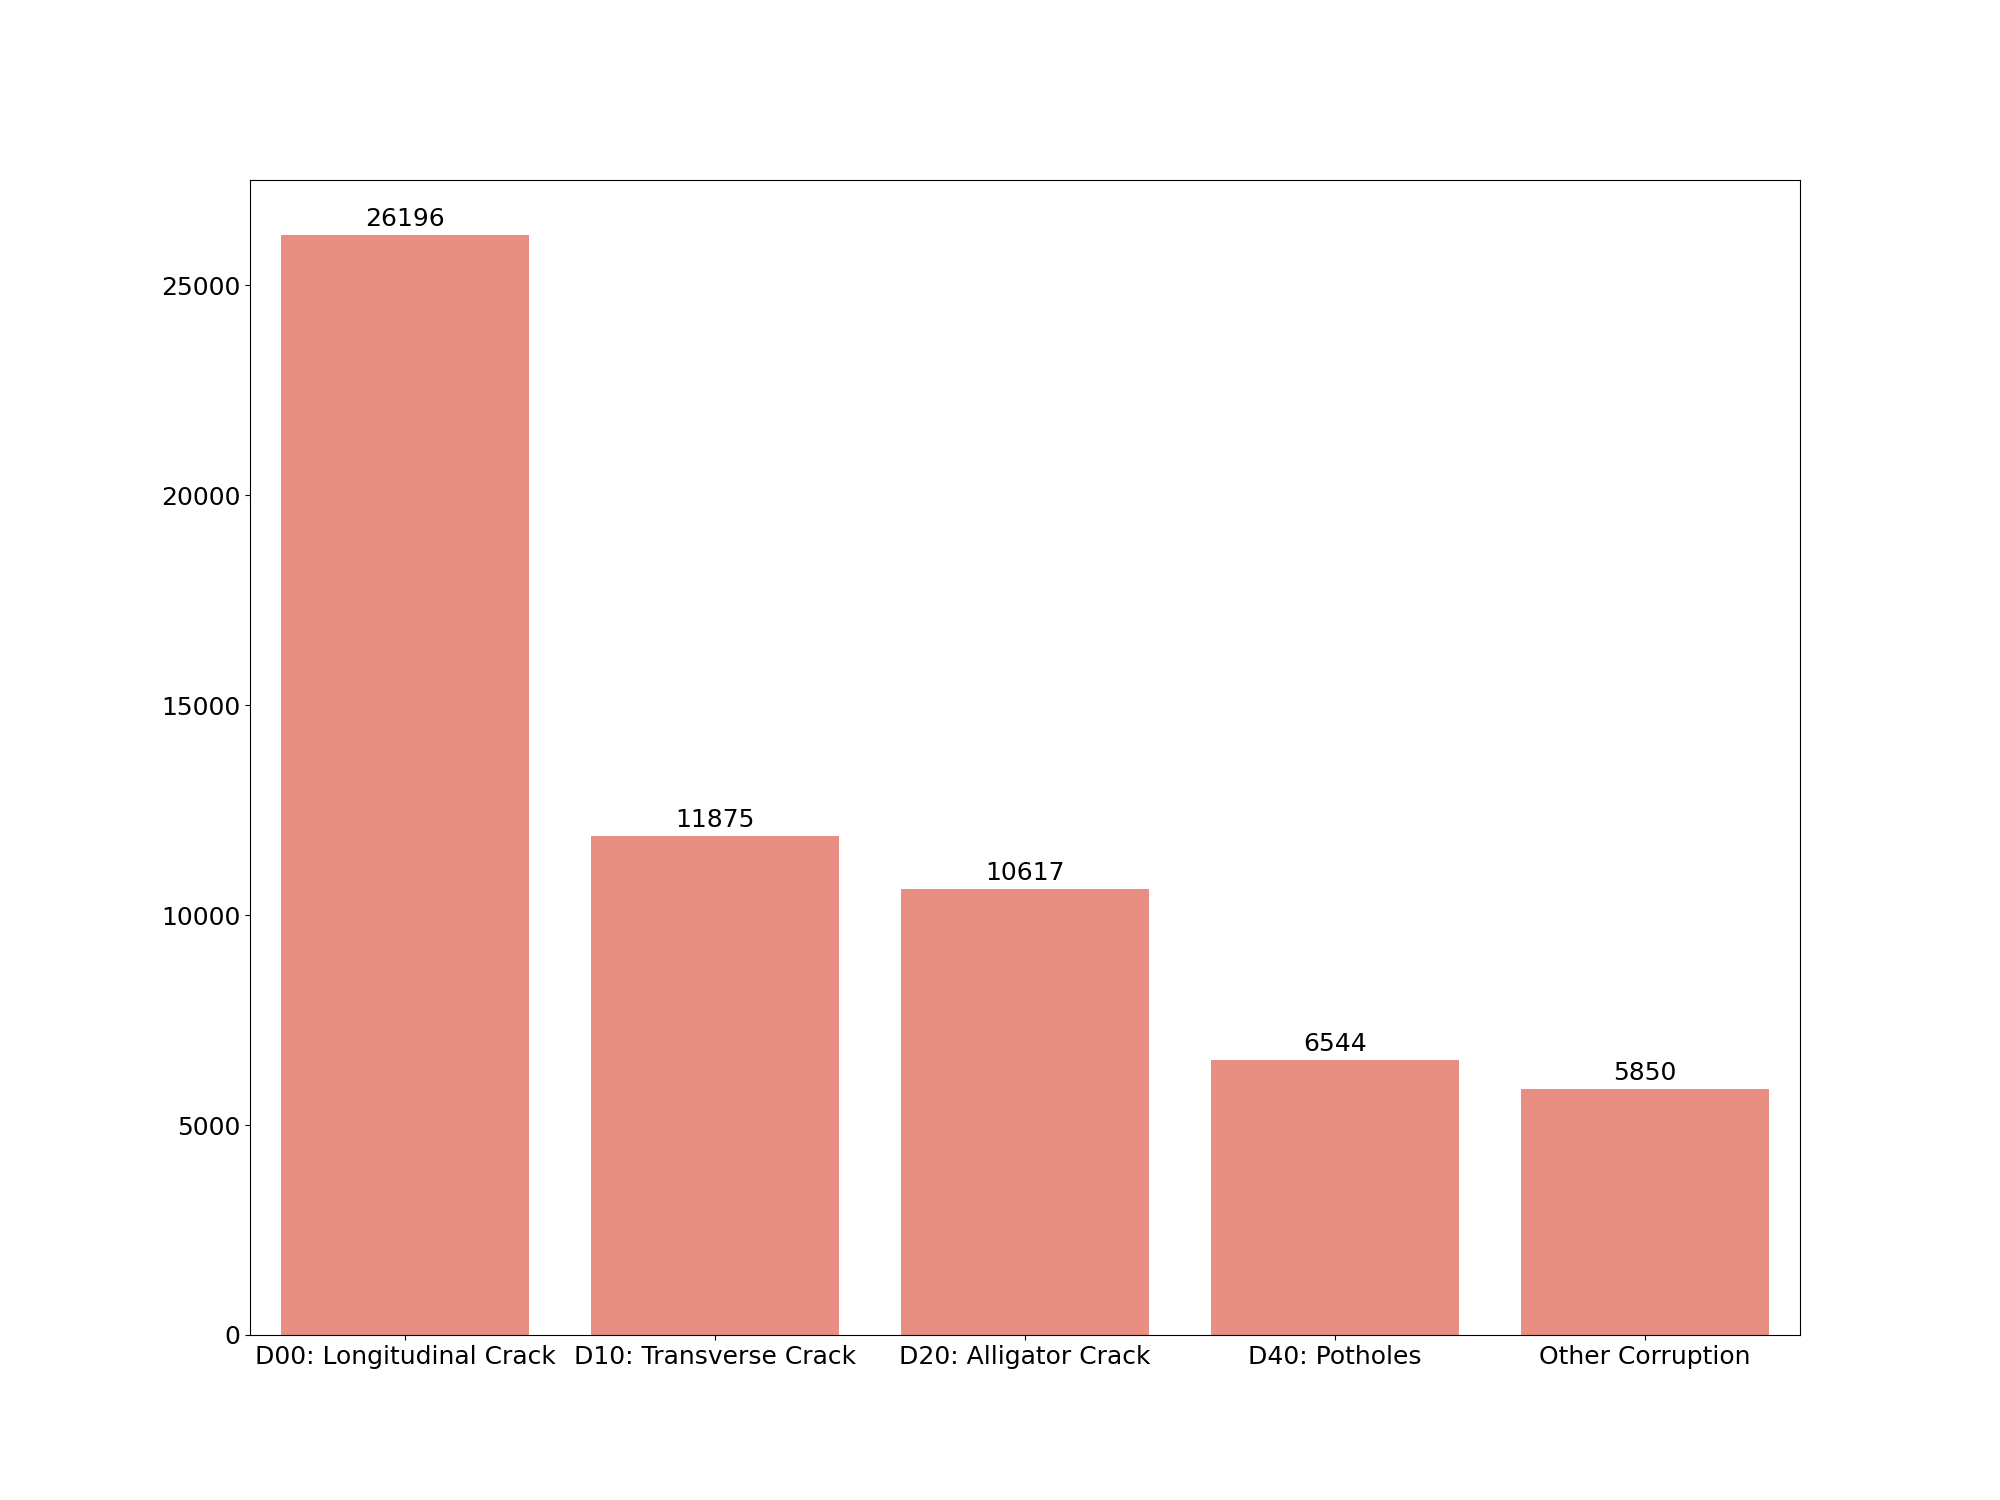
\includegraphics[width=0.8\textwidth]{graphs/datasetNinja_class_count_bar.png}
    \caption{Número de anotaciones por clase en los datos de la CRDDC2022.}
    \label{fig:datasetNinja_class_count_bar}
\end{figure}


\subsection{¿Cómo son las imágenes?}
Las imágenes han sido capturadas con sistemas muy diferentes dependiendo del subconjunto al que pertenecen. Esto junto con la diversidad de los entornos en los que se han tomado las imágenes, hace que las imágenes tengan una gran variabilidad en cuanto a calidad, resolución, iluminación, etc. En la tabla \ref{tab:dataset_info} se puede ver un resumen de la información sobre las imágenes de los datos de la CRDDC2022.

% Tabla explicativa de Region, Vehiculo, Dispositivo utilizado para capturar las imágenes, Resolución de las imágenes, Número de imágenes y Número de anotaciones
\begin{table}[H]
    \centering
    \begin{tabular}{|c|c|c|c|c|c|}
        \hline
        \textbf{Región} & \textbf{Vehículo} & \textbf{Dispositivo} & \textbf{Resolución} & \textbf{Nº Imágenes} & \textbf{Nº Anotaciones} \\
        \hline
        China & Motocicleta & Smartphone & 512x512 & 2477 & 4650 \\
        China & Dron (DJI M600 Pro) & Drone Camera & 512x512 & 2401 & 3068 \\
        República Checa & Vehículo & Dashcam & 600x600 & 3538 & 1745 \\
        India & Vehículo & Dashcam & 720x720 & 9665 & 6831 \\
        Japón & Vehículo & Dashcam & 600x600 & 13133 & 16470 \\
        Noruega & Vehículo & High-resolution Cameras & 4040x2035 & 10201 & 11229 \\
        Estados Unidos & Vehículo & Google Street View & 640x640 & 6005 & 11014 \\
        \hline
    \end{tabular}
    \caption{Información sobre las imágenes de los datos de la CRDDC2022.}
    \label{tab:dataset_info}
\end{table}

En la tabla se puede ver que las imágenes de Noruega van a tener que ser redimensionadas para poder trabajar con ellas, ya que tienen una resolución mucho mayor que el resto de imágenes y que no es necesaria para el entrenamiento de nuestros modelos. También se puede ver que hay una gran variabilidad en los métodos de captura de imagen. Tendremos que tener en cuenta esta variabilidad a la hora de entrenar nuestros modelos, ya que si estos no son capaces de generalizar bien, podrían tener problemas a la hora de detectar daños en el pavimento en imágenes que no se parezcan a las del conjunto de entrenamiento, más adelante veremos cómo abordar este problema.

En la figura \ref{fig:example_images_region} se muestran algunas imágenes de los datos de la CRDDC2022 sin sus correspondientes anotaciones. Nótese la diferencia en la calidad y resolución de las imágenes, y la variabilidad en los entornos en los que se han tomado.

% Añadimos las imágenes example_images_region de la carpeta images
\begin{figure}[H]
    \centering
    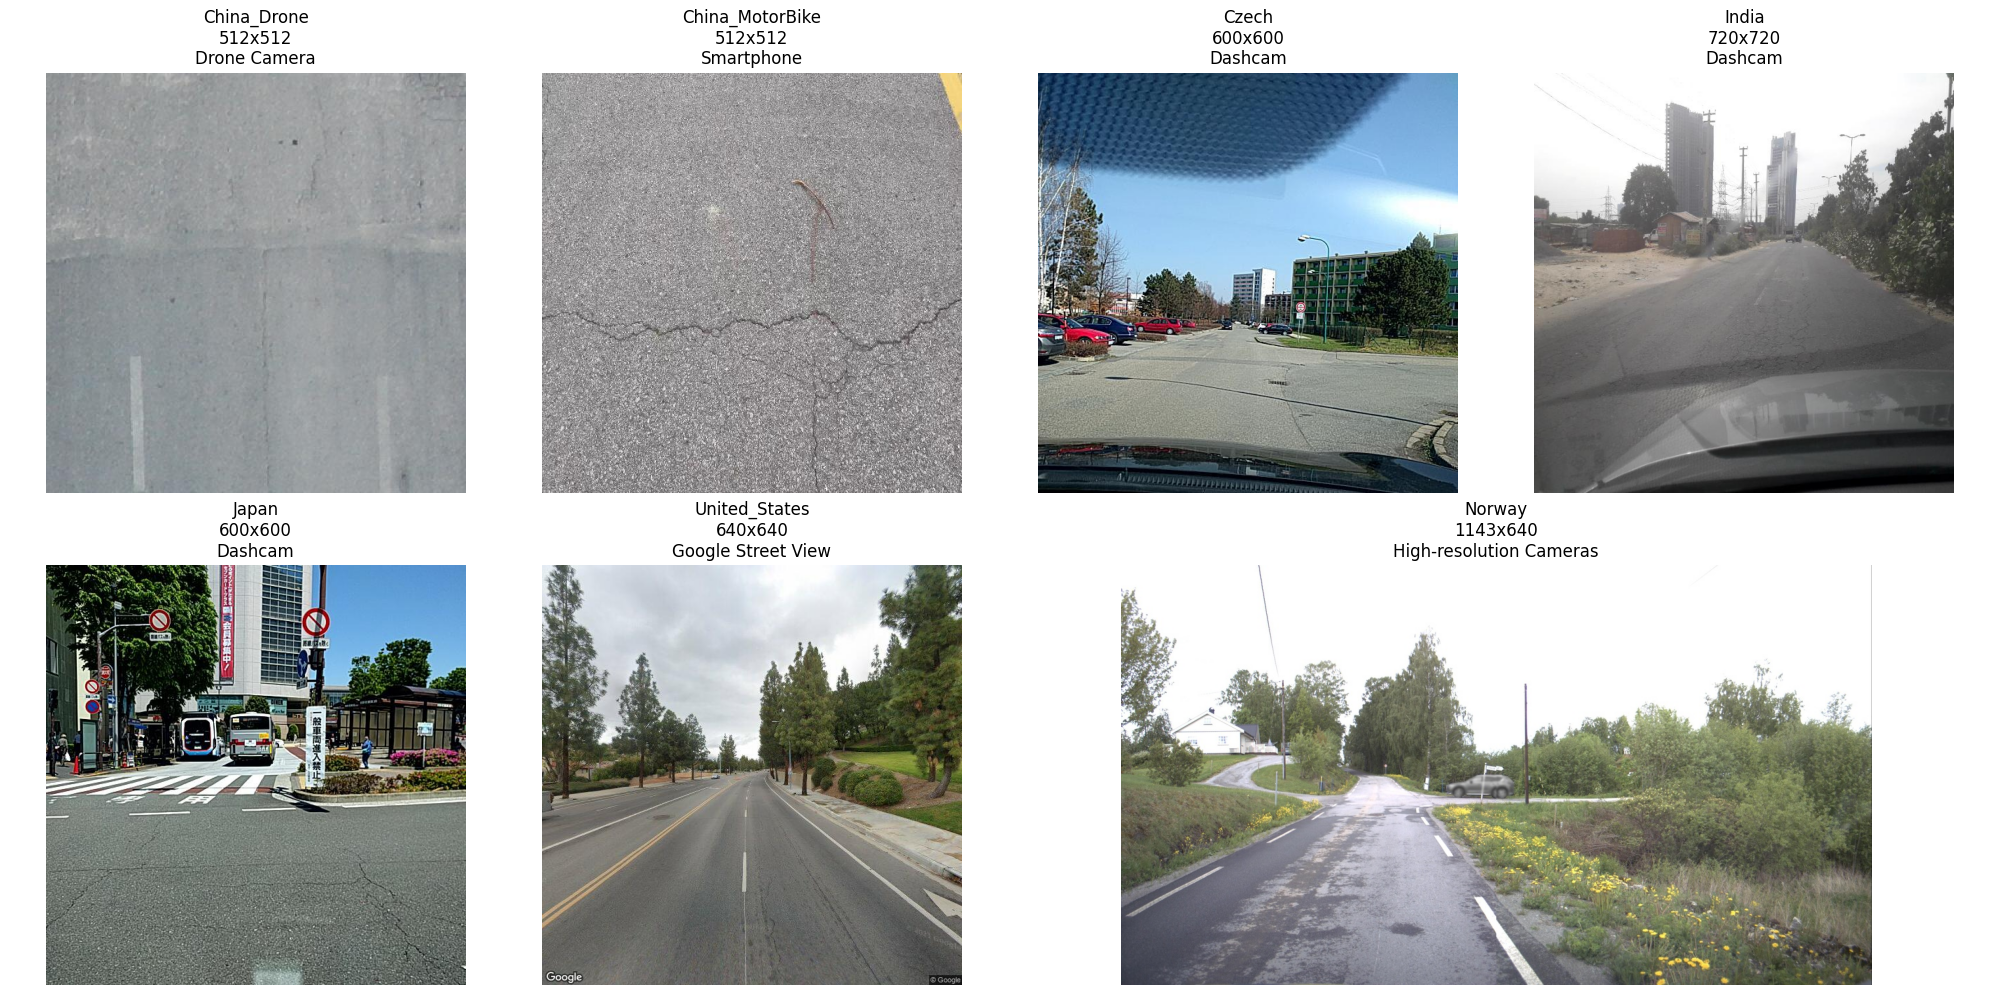
\includegraphics[width=1\textwidth]{img/example_images_regions.png}
    \caption{Ejemplos de imágenes de los datos de la CRDDC2022.}
    \label{fig:example_images_region}
\end{figure}